\chapter{\IfLanguageName{dutch}{Integratie van Voorgetrainde Pose Estimation Modellen}{Datacollection and Labeling}}%
\label{ch:poseestimation}

\subsection{Doelstelling}
Voor de pose estimation in dit onderzoek is gekozen voor het gebruik van het ViTPose model. Dit voorgetrainde model is bijzonder geavanceerd en staat bekend om zijn uitzonderlijke nauwkeurigheid en complexiteit in het identificeren van specifieke lichaamshoudingen. Het ViTPose model is specifiek ontworpen om uitdagingen in pose estimation te overwinnen door gebruik te maken van state-of-the-art technologieën en een omvangrijke trainingsdataset.

\subsection{Methoden}
\begin{itemize}
  \item \textbf{Trainingsdetails:} Voor de pose estimation is gekozen voor een voorgetraind ViTPose model, dat bekend staat om zijn hoge nauwkeurigheid en complexiteit. Dit model is getraind op de APT-36K dataset, een grootschalige dataset specifiek voor animal-pose estimation, bestaande uit 36,000 handmatig gelabelde foto's van 30 verschillende diersoorten. Het model identificeert 17 keypoints per dier, waaronder ogen, neus, nek, staart, schouders, ellebogen, knieën, heupen en poten. Het model is getraind op een indrukwekkende setup van 8 NVIDIA Tesla V100 (32G) GPUs. Deze krachtige GPU's bieden de noodzakelijke rekenkracht om grote en complexe datasets te verwerken, wat essentieel is voor de ontwikkeling van een robuust en nauwkeurig pose estimation model.
  \item \textbf{Alternatieve trainingspogingen:} Er zijn experimenten uitgevoerd met voorgetrainde modellen op de COCO dataset en de APT10K dataset. Echter, uit deze tests bleek dat het model getraind op de APT-36K dataset de beste resultaten leverde voor de specifieke behoeften van dit onderzoek, vanwege de grotere variëteit en specialisatie in dierposes.
  \item \textbf{Beslissing tegen eigen training:} Gezien de complexiteit en de geavanceerde aard van het ViTPose model en de vereiste rekenkracht, werd besloten om het voorgetrainde model te gebruiken zonder verdere aanpassing of hertraining. Het zelf trainen van een dergelijk model zou niet alleen een vergelijkbare of betere dataset en vergelijkbare hardware vereisen, maar ook een diepgaande expertise in machine learning en computervisie. Bovendien is het onwaarschijnlijk dat een nieuw trainingsregime significant zou verbeteren op de reeds uitzonderlijke prestaties van het ViTPose model, gezien de kwaliteit en schaal van de initiële training.
  \item \textbf{Modelintegratie en dataflow:} Eerst wordt objectdetectie uitgevoerd om de koeien in de videobeelden te identificeren en te lokaliseren. Voor elke gedetecteerde koe wordt een bounding box gecreëerd. Binnen deze bounding box gebruikt het ViTPose model de pose estimation technologie om de keypoints van het skelet van de koe te voorspellen.
  \item \textbf{Gedragsanalyse op basis van keypoints:} Specifieke algoritmes werden ontwikkeld om het gedrag van de koeien te interpreteren aan de hand van de posities van de keypoints. Bijvoorbeeld, de positie van de nek kan aangeven of een koe aan het grazen is, en de afstand tussen de heupen en poten kan aangeven of een koe ligt. Door de grootte van elke poot te berekenen ten opzichte van de lengte van de koe en de hoeken tussen elke poot en de nek te analyseren, kon gedrag nauwkeuriger worden vastgesteld dan met enkel objectdetectie.
\end{itemize}

\subsection{Resultaten}
\begin{itemize}
  \item \textbf{Integratie van technologieën:} De integratie van objectdetectie en pose estimation modellen resulteerde in een krachtig systeem dat in staat is om gedetailleerd gedrag en lichaamshoudingen van koeien te analyseren.
  \item \textbf{Betrouwbaarheid van gedragsclassificatie: } De combinatie van deze twee modellen verhoogt de betrouwbaarheid van de gedragsclassificatie aanzienlijk. Wanneer beide modellen hetzelfde gedrag suggereren, wordt de nauwkeurigheid van de classificatie effectief verhoogd naar een zeer hoog betrouwbaarheidsniveau.
  % \item \textbf{Voorbeeld object detectie gedrag (links) vs pose estimation gedrag (rechts). } Duidelijk verbetering in gedrag voorspelling door diepere analyse van lichaamshoudingen met de pose estimation. 
  % \newline 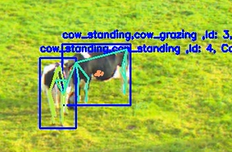
\includegraphics[width=\linewidth]{pose_werkend_voorbeeld.png}
  \item \textbf{Pretrained on COCO dataset:} \newline 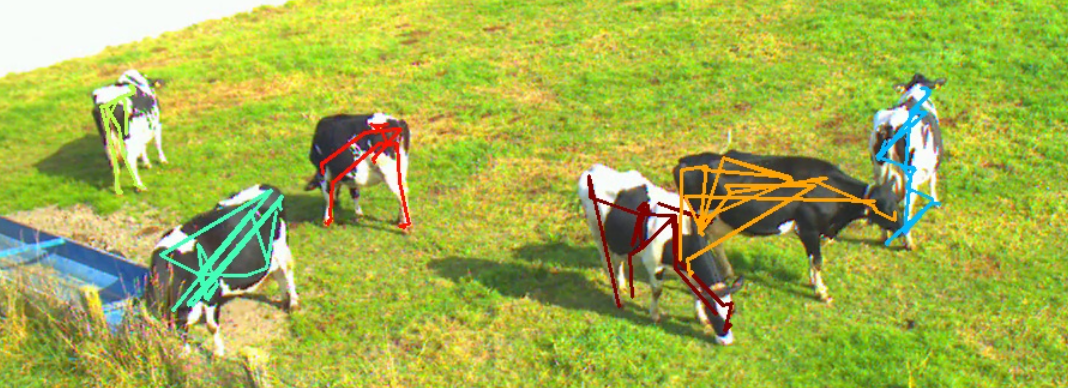
\includegraphics[width=\linewidth]{pose_cocoposes.png}
  \item \textbf{Pretrained on APT-36K dataset:} \newline 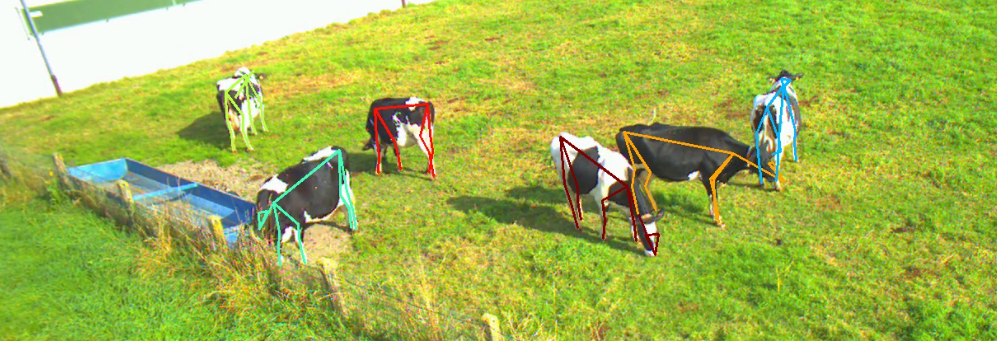
\includegraphics[width=\linewidth]{pose_apt36k.png}
\end{itemize}